\let\negmedspace\undefined
\let\negthickspace\undefined
\documentclass[journal]{IEEEtran}
\usepackage[a5paper, margin=10mm, onecolumn]{geometry}
\usepackage{lmodern} % Ensure lmodern is loaded for pdflatex
\usepackage{tfrupee} % Include tfrupee package

\setlength{\headheight}{1cm} % Set the height of the header box
\setlength{\headsep}{0mm}     % Set the distance between the header box and the top of the text

\usepackage{gvv-book}
\usepackage{gvv}
\usepackage{cite}
\usepackage{amsmath,amssymb,amsfonts,amsthm}
\usepackage{algorithmic}
\usepackage{graphicx}
\usepackage{textcomp}
\usepackage{xcolor}
\usepackage{txfonts}
\usepackage{listings}
\usepackage{enumitem}
\usepackage{mathtools}
\usepackage{gensymb}
\usepackage{comment}
\usepackage[breaklinks=true]{hyperref}
\usepackage{tkz-euclide} 
\usepackage{listings}
\usepackage{gvv}                                        
\def\inputGnumericTable{}                                 
\usepackage[latin1]{inputenc}                                
\usepackage{color}                                            
\usepackage{array}                                            
\usepackage{longtable}                                       
\usepackage{calc}                                             
\usepackage{multirow}                                         
\usepackage{hhline}                                           
\usepackage{ifthen}                                           
\usepackage{lscape}
\begin{document}

\bibliographystyle{IEEEtran}
\vspace{3cm}

\title{9.1.8}
\author{EE24BTECH11005 - Arjun Pavanje}
% \maketitle
% \newpage
% \bigskip
{\let\newpage\relax\maketitle}
\textbf{Question:}
Solve the differential equation $y^{\prime}+y=e^x$ with initial conditions $y\brak{0}=\frac{1}{2}$
\solution\\
\textbf{Theoretical Solution:}\\
This is a linear differential equation of the first order.
\begin{align}
  \frac{dy}{dx} + y = e^x\\
\end{align}
Finding integrating factor 
\begin{align}
  &e^{\int 1dx}\\
  &=e^x
\end{align}
Multiplying both sides of $\brak{2}$ with integrating factor,
\begin{align}
  \frac{dy}{dx}\brak{e^x} + ye^x = e^{2x}\\
  \frac{d\brak{ye^x}}{dx}=e^{2x}\\
  ye^x=\frac{e^{2x}}{2}+c\\
  y=\frac{e^x}{2}+ce^{-x}
\end{align}
On substituting initial conditions we get,
\begin{align}
  y=\frac{e^x}{2}
\end{align}

\textbf{Computational Solution:}\\
Aim is to find a computational solution to the differential equation using trapezoidal law.
\begin{align}
  y^{\prime}+y&=e^x
\end{align}
Integrating by setting limits after discretizing,
\begin{align}
  \int_{y_n}^{y_{n+1}}dy&=\int_{x_n}^{x_{n+1}}-y dx +\int_{x_n}^{x_{n+1}} e^x dx
\end{align}
We can solve the two integrals on the $R.H.S$ by using trapezoid method
\begin{align}
  \int_{x_n}^{x_{n+1}}ydx&= h\sbrak{\frac{y\brak{x_{n+1}}+y\brak{x_n}}{2}}\\
  \int_{x_n}^{x_{n+1}}e^xdx&= h\sbrak{\frac{e^{x_{n+1}}+e^{x_n} }{2}}
\end{align}
Substituting into equation $\brak{11}$
\begin{align}
  y_{n+1}-y_{n}&=-h\brak{\frac{y_{n+1}+y_{n}}{2}}+h\brak{\frac{e^{x_{n+1}}+e^{x_n}}{2}}\\
  y_{n+1}\brak{2+h}&=y_n\brak{2-h}+he^{x_n}\brak{\frac{1+e^h}{2}}
\end{align}
The general difference equation comes out to be,
\begin{align}
  y_{n+1}&=y_n\brak{\frac{2-h}{2+h}}+e^{x_n}h\brak{\frac{1+e^h}{2\brak{2+h}}}
\end{align}

Below is a comparission between Simulated Plot and Theoretical Plot.
\begin{figure}[h!]
   \centering
   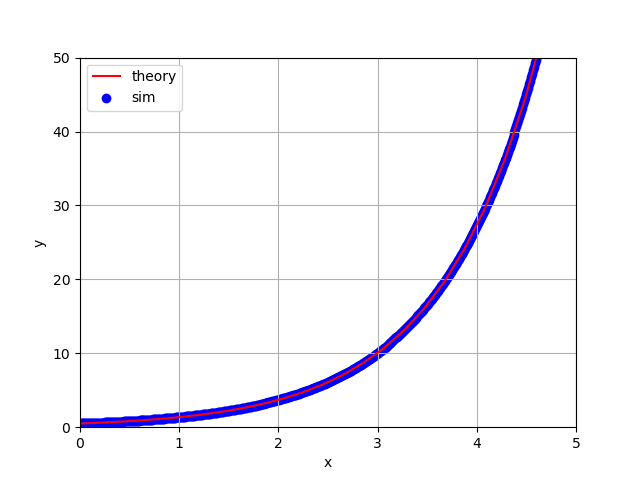
\includegraphics[width=1\columnwidth]{figs/fig.png}
   \caption{Computational vs Theoretical solution of $ \frac{dy}{dx}=-\frac{y^2+y+1}{x^2+x+1}$}
   \label{stemplot}
\end{figure}
\end{document}
